\namedsection{Analyse der Drittsysteme}{J}
Zum Start des Projektes wurden bereits anfänglich drei Drittsysteme genannt die für eine weitergehende Analyse für Statistance von Interesse sein könnten. Demzufolge haben wir uns mit den Drittsystemen Sage, Navision und QDX auseinandergesetzt. Da Sage beim Pilotkunden zur Anwendung kommt haben wir bei der Analyse einen besonderen Fokus auf dieses System gelegt.

Generell sollte man im Hinterkopf behalten das speziell Sage und Navision stark anpassbare ERP-Systeme sind und es teils größere Versionsunterschiede innerhalb dieser Systeme gibt. Dementsprechend kann sich die Ausgestaltung und die Datenvollständigkeit je nach Kunde drastisch unterscheiden.
Aus diesem Grund wurde versucht für Navision ein eher allgemeines Bild des Systems zu erfassen. Bei Sage wird wiederum vermehrt auch auf die Spezifika der Sage 100 Version eingegangen.

\namedsubsection{Sage}{J}
Wenn wir von Sage sprechen, ist stets das ERP System Sage 100 von gleichnamiger Softwarefirma gemeint. Die Version Sage 100 ist der Vorgänger der Versionen Sage 200 Evolution, Sage 300 Cloud und Sage X3 und ist sowohl als Cloud, als auch als lokale (On-Premise) Lösung verfügbar.

Im Kontext dieses Projektes haben wir uns ausschließlich mit der On-Premise Version befasst, da dieses auch bei dem Pilotkunden von Statistance lokal verwendet wird.

Das Sage System besteht aus folgenden Komponenten:

\begin{itemize}
  \item \textbf{Rich Client: } Das ERP System selbst ist als Rich Client Applikation implementiert, es wird also jegliche Applikationslogik im Prozess des Clients ausgeführt. Die Kommunikation zwischen Client und Applikationsserver findet über das Sage-eigene Protokol S-Data statt, welches im folgenden Kapitel ausführlich beschrieben wird.  Ein beispielhaftes User-Frontend ist in Abb.\ref{fig:sage_screenshot} zu sehen.

  \item \textbf{Applikationsserver: } 
  Da es sich um eine Rich Client Anwendung handelt muss der Applikationsserver für die Einhaltung der ACID Prinzipien, also insbesondere konsistente Datenhaltung kümmern. Daher entfallen auf ihn die zusätlichen Aufgaben der Isolierung einzelner Anwendungen für die parallele Ausführung und das Pooling von Applikationskernen \cite{sageadministrationshandbuch}.
  \item \textbf{Datenbank: } Als Datenbank wird eine MSSQL Datenbank verwendet, welche mindestens die Version \"Microsoft SQL Server 2008\" oder neuer verwendet.
\end{itemize}

\begin{figure}[!h]
\centering
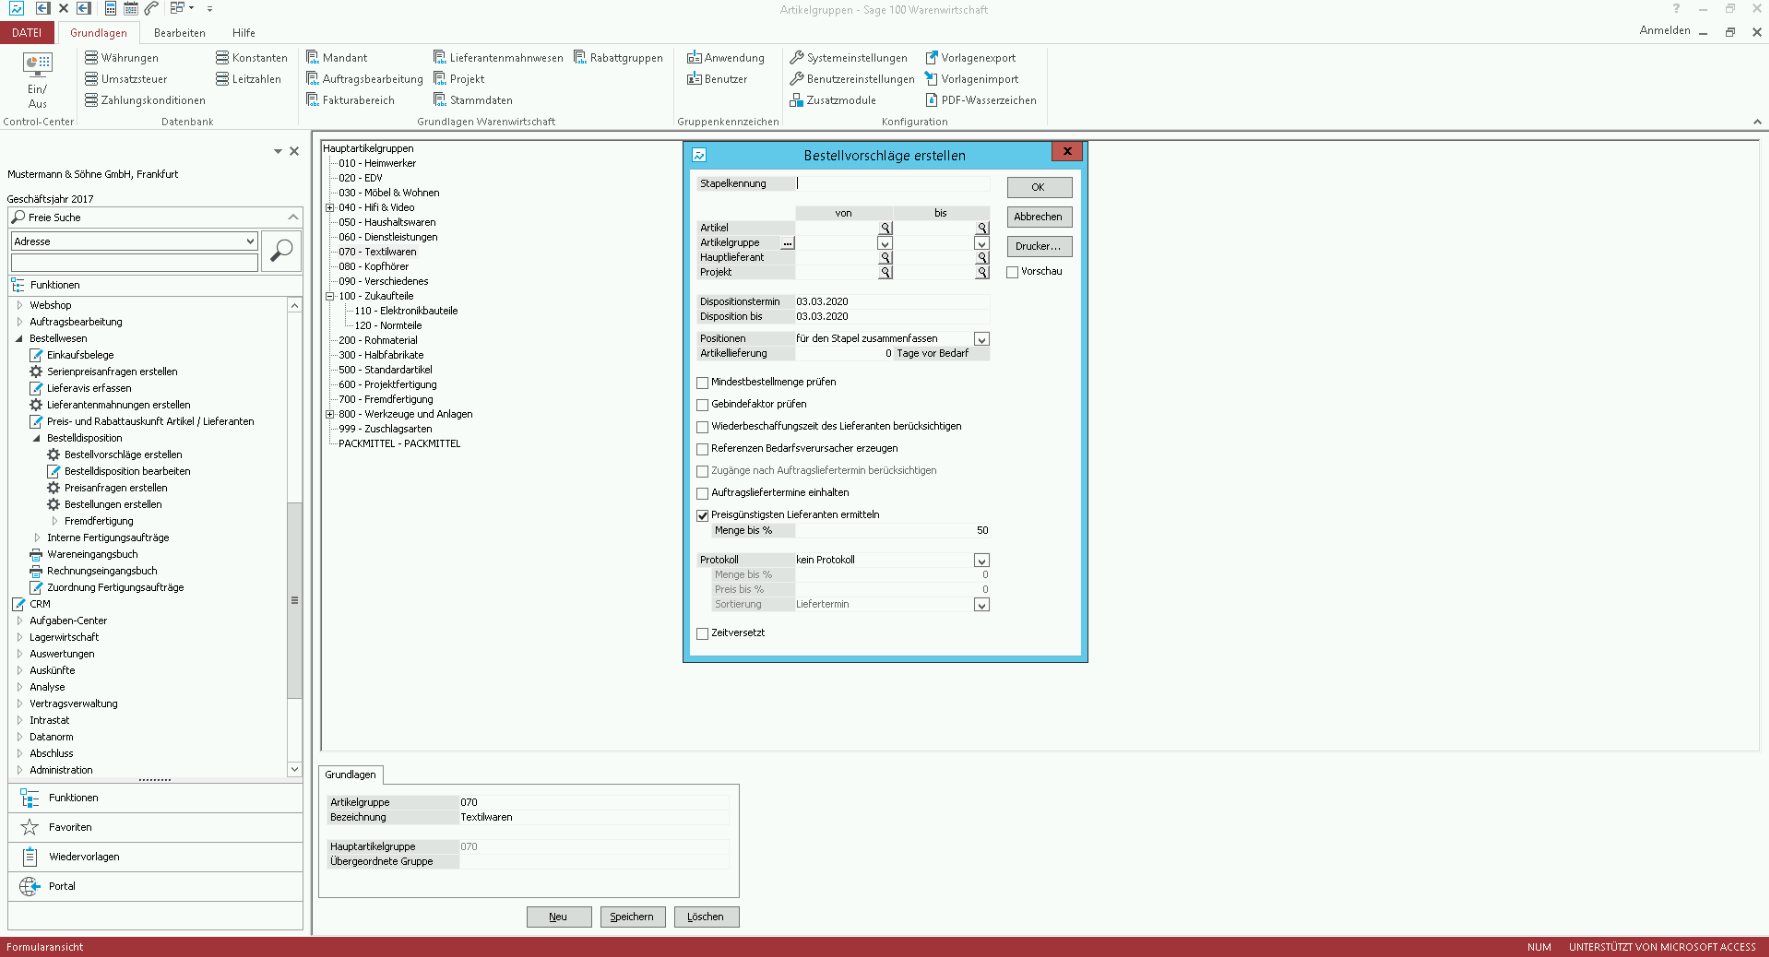
\includegraphics[width=13.5cm]{images/03_SAGE/Sage_100_Screenshot.png}
\caption{Rich Client Interface auf einem Windows Server}
\label{fig:sage_screenshot}
\end{figure}

\subsubsection*{Module}

Innerhalb des Sage 100 Systems existieren verschiedene Module, welche sich in die Kernmodule (Finanzwesen, Warenwirtschaft und Produktion) und Zusatzmodule einteilen lassen. Diese Module sind wiederum in Einzelbereiche aufgeteilt (z.B Einkauf und Verkauf). Für Statistance ist in diesem Kontext insbesondere der Einkaufsbereich des Warenwirtschaftsmoduls relevant, da dieser die Wareneingänge und Belege beinhaltet, für welche Sie ihre statistischen Vorhersagen treffen.

\namedsubsection{Sage 100 SData}{J}
Die SData Spezifikation beschreibt ein von Sage entwickeltes Protokoll zum lesen, ändern, erstellen und löschen von Daten aus dem ERP-System~\cite{sdatadocu}. Dieses Protokoll beschreibt den Aufbau der REST-Schnittstelle und wie die Kommunikation zwischen Consumer und Provider auszusehen hat. Die Daten werden hierbei in Form von Atom Feeds, ein Standard im XML-Format~\cite{atomfeed}, übertragen. Die Webservices für SData wiederum werden bei der Installation von Sage 100 automatisch mit installiert und sind standardmäßig aktiviert \cite{sageadministrationshandbuch}. Die Abbildung \ref{fig:sdataservicesadmin} zeigt hierbei alle aktiven SData Services bei einer Standardinstallation von Sage 100 an inklusive Anzahl der Zugriffe.

\begin{figure}[!h]
\centering
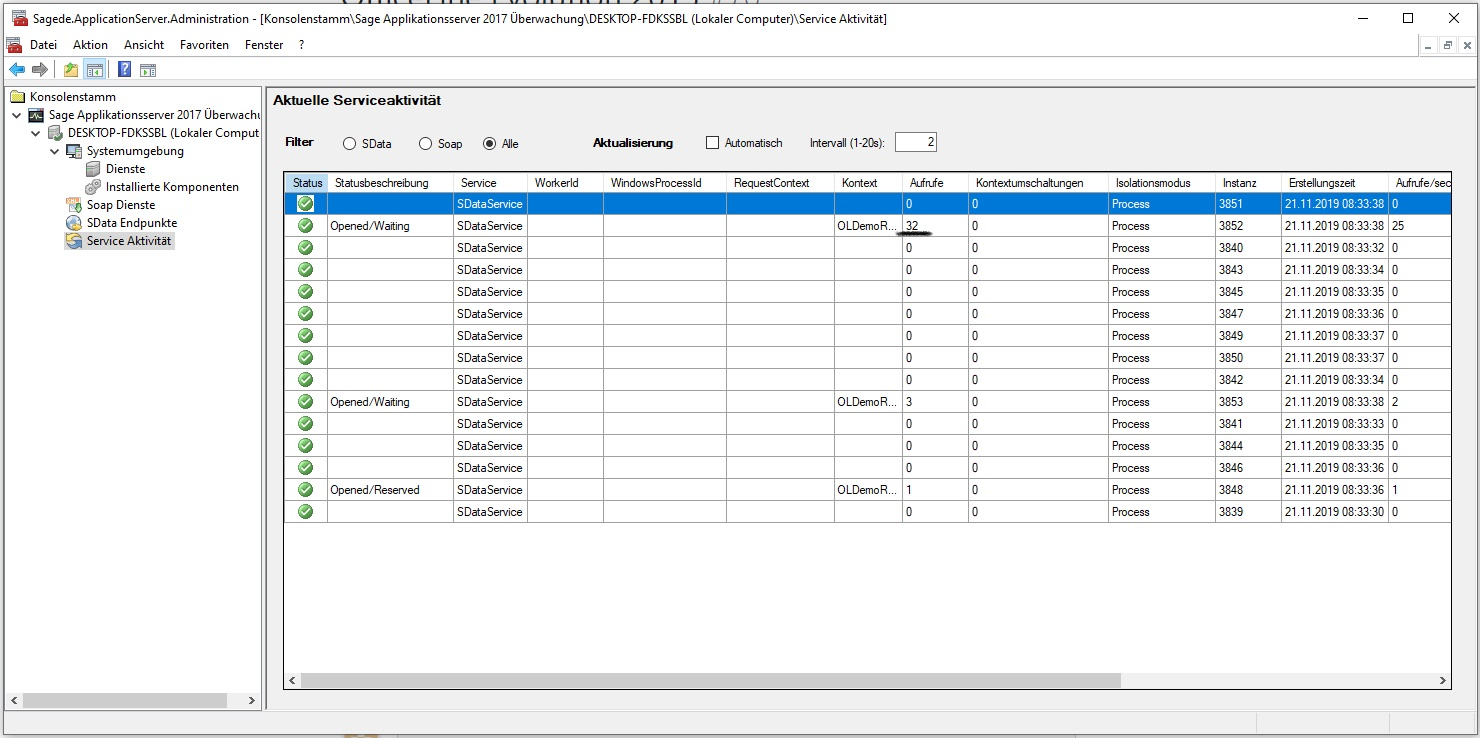
\includegraphics[width=12cm]{images/0x_requirement_analysis/sage-admin-sdata.png}
\caption{Adminpanel SData Services}
\label{fig:sdataservicesadmin}
\end{figure}

Interessant ist eine Untersuchung von SData für uns gewesen, weil es die Möglichkeit bieten könnte Daten sicher zurück in die Datenbank einzuspielen ohne sie fehlerhaft zu bespielen. Ebenfalls wäre die Schnittstelle eher für Fälle geeignet in denen die Dienste von Statistance als SaaS in Anspruch genommen werden. Bei einer Cloud-Lösung müssen Daten über das Internet übertragen werden. Das erstellen eines Adapters würde somit bei Nutzung von SData anteilig entfallen.

Die ursprüngliche Annahme ist gewesen, dass alle Endpunkte von SData grundsätzlich alle CRUD-Operationen erlauben. Dies fußte auf die initiale Begutachtung mehrerer Endpunkte bei denen das Löschen und Ändern der Daten problemlos möglich ist. Jedoch stellte sich diese Annahme nach Betrachtung der für uns wichtigsten Endpunkte später als Irrtum heraus.

* Beschreibung Aufbau Payload
** Attribute für Operatoren
** Beispielresponse

\begin{figure}[!h]
\centering
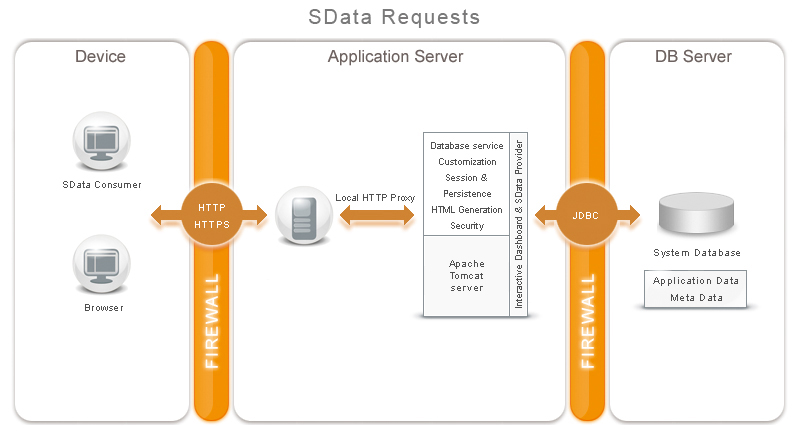
\includegraphics[width=12cm]{images/0x_requirement_analysis/sdata_requests_arch.png}
\caption{SData Integration in Sage~\cite{sdata_requests}}
\label{fig:sdataintegrationsage}
\end{figure}

Fehlermeldungen bei der ungültigen Nutzung der SData Services lassen darauf schließen, dass Sage intern verschiedene Safeguards für die Nutzung der Schnittstellen enthält um die ordnungsgemäße Funktionsweise der Datenbank zu gewährleisten. Auch eine Betrachtung der Integration von SData in den Applikationsserver von Sage bestätigen diesen Eindruck wie auf Abbildung \ref{fig:sdataintegrationsage} zu entnehmen ist.

\subsubsection*{Security}

Man hat die Möglichkeit die Authentifizierung entweder im Basic oder Digest-Modus auszuführen \cite{sdatadocu_auth}. Im ersterem Fall empfiehlt es sich den Datenaustausch mit SSL zu verschlüsseln weil die Login-Daten sonst sehr einfach auf dem Übertragungsweg abgegriffen werden können (z.B. über Man-in-the-Middle-Angriffe). Der andere Modus erfordert im Gegensatz dazu mehr Aufwand für die Umsetzung. Basic scheint in den vorhandenen Consumer-Clients enthalten zu sein. Beim anderen Modus ist es noch unklar.
Darüber hinaus findet sich im Handbuch die Erwähnung eines STS (Token Service) für SData, dass für die Absicherung von Verbindungen ebenfalls relevant sein dürfte \cite{sageadministrationshandbuch} (S. 51). Jedoch entsprechen diese Methoden nicht mehr den heutzutage empfohlenen Verfahren laut der OWASP \cite{owasp_authentication}.

Ebenfalls relevant ist die Autorisierung der Ressourcen. Über unterschiedliche Benutzerberechtigungen sollte es auch möglich sein den Zugriff einzuschränken bzw. auf Read-only zu setzen. Im Handbuch findet sich dazu eine Anleitung wie man den Zugriff je Benutzer auf bestimmte Bereiche beschränken kann \cite{sageadministrationshandbuch} (S. 33 f.).

\subsubsection*{Vorteile}
\begin{itemize}
    \item Es gibt bereits Consumer-Clients für C\# und JavaScript\footnote{Siehe https://github.com/Sage/SDataCSharpClientLib und https://github.com/Sage/SDataJavaScriptClientLib}
    \item REST-like Schnittstelle mit CRUD Capability
    \item keine direkte Datenbankanbindung nötig und “Bidirektional”
    \item Schemata können direkt vom Webservice abgefragt werden (Validierung)
    \item Die Schnittstelle ist auch Hypermedia-Driven, d.h. alle Daten werden immer mit navigierbaren Links ausgeliefert
    \item Automatisch SSL bei Installation \cite{sageadministrationshandbuch} (S. 22 und S. 26)
    \item Im Gegensatz zum direkten Datenbankzugriff Safeguards für das Löschen, Ändern und Hinzufügen von Daten vorhanden
\end{itemize}

\subsubsection*{Nachteile}
\begin{itemize}
    \item sehr wenig dokumentiert
    \item nicht alle Daten lassen sich erstellen
    \item Authentifizierung entspricht nicht mehr den heutzutage gängigen Standards \cite{owasp_authentication}
\end{itemize}

Wie man Einstellungen am SData Provider vornehmen kann ist im Handbuch dokumentiert \cite{sageadministrationshandbuch} (S. 57 ff., S. 36 f.).
Das Sage 100 ERP-System erlaubt es auch SOAP-Services zu installieren. Wie das abzulaufen hat kann unter Soap-Service Installation im Handbuch nachgesehen werden \cite{sageadministrationshandbuch} (S. 27).

\subsubsection*{Aufbau REST-API}
Alle Links beziehen sich momentan auf die derzeit laufende Demo-Instanz bei Statistance.
Aus uns noch nicht nachvollziehbaren Gründen antwortet der Linux Postman-Client auf eine Anfrage mit einer Server-Fehlermeldung. Es müsste in diesem Fall geklärt werden woran es genau liegt. Die Windows-Variante stellt keinerlei Probleme dar.

Meistens ausgehend von der baseurl 
\begin{quotation}
    https://app.statistance.de:5493/sdata/ol/Default/OLDemoReweAbfD;123
\end{quotation}
werden wir nachfolgend einige wichtige Endpunkte der SData Schnittstelle aufführen.

\begin{description}
    \item [https://app.statistance.de:5493/sdata/ol/Default]
    Enthält die Endpoint-URLs für die vorhandenen Datenbanken, in der Sage 100 Demo-Version werden jeweils zwei angelegt
Für uns erstmal relevant dürfte die URL zur Beispieldatenbank sein
ol steht vermutlich für Office Line
    \item [<baseurl>]
    Hier werden alle erreichbaren Endpunkte für die Beispieldatenbank aufgeführt
    Nachfolgend am Beispiel des Endpoints Adressen werden wir auf den groben Aufbau dieser Endpunkte eingehen. Der Aufbau ist für alle anderen Endpoints gleich.
    \item [<baseurl>/Adressen]
    Listet alle vorhandenen Adressen der Datenbank auf
    \item [<baseurl>/Adressen/\$schema]
    Enthält das XML Schema für Adressen
Zudem kann man anhand der Attribute sme:canGet(|Put|Post|Delete) im ersten xs:element-Tag erkennen was man mit der Ressource alles anstellen kann
    \item [<baseurl>/Adressen/\$template]
    Beispiel-Payload für zum Beispiel einem Put oder Post-Requests
    \item [<baseurl>/Adressen?where=\$updated gt @2019-12-19T22:00Z@]
    Mithilfe des where-Querys lassen sich Abfragen filtern
In unserem Beispiel sollen nur Adressen angezeigt werden die seit dem im @-Zeichen umschlossenem Datetime zuletzt geupdated wurde
Unglücklicherweise funktioniert das gegenwärtig nicht, weil das updated-Feld einer Ressource immer dem Requestzeitpunkt entspricht
Meiner Meinung nach kann das kein normales Verhalten sein, vielleicht lässt es sich in den Sage Einstellungen irgendwie beheben
Alle möglichen Operatoren, Funktionen und Spezialvariablen lassen sich in http://sage.github.io/SData-2.0/pages/core/0212/ einsehen
    \item [<baseurl>/Adressen?where=Adressen.ADR\_Gruppe eq 'MA']
    Ein weiteres Beispiel für die Nutzung des where-Querys
Query entspricht: Wähle nur Adressen aus die zur Adressgruppe der Mitarbeiter gehören
\end{description}

\namedsubsection{Navision}{J}
Wenn wir von Navision sprechen ist stets das ERP-System von Microsoft gemeint. Auch wenn es schon seit längerem Microsoft Dynamics NAV oder seit neuestem Microsoft Dynamics 365 Business Central heißt. In diesem Dokument behandeln wir: 
Wie sich Navision über die Zeit entwickelt hat,
welche “Objekte” in Navision existieren und warum das wichtig für uns ist,
wie man Zugriff auf die Daten von Navision erhält (welche Schnittstellen, Webhooks, etc.),
welche von Statistance benötigten Informationen von Navision abgedeckt werden,
und wie man es sinnvoll in unsere Architektur integrieren könnte.

\subsubsection*{Versionen}
\begin{enumerate}
\item 1995 Erste Version (Navision Financials 1.0) für ein Windows Betriebssystem (Windows 95) veröffentlicht
\item 2002 Microsoft kauft das Navision Unternehmen
\item 2005 Microsoft benennt Navision zu Dynamics NAV um
\item 2008 Mit Dynamics NAV 2009 werden alle internen Vorgänge von Dynamics NAV von den Clients getrennt und in ein Application Server Service ausgekoppelt
\item 2012 Mit Dynamics NAV 2013 kommt OData Support für Queries dazu (erst ab Dynamics NAV 2013 R2 mit Schreibzugriff) und es wird nur noch der Microsoft SQL Server als DBMS verwendet
\item 2018 Aktiver Support für alle Versionen vor 2009 läuft aus und das ERP-System firmiert nun unter den Namen Dynamics 365 Business Central
\end{enumerate}

\subsubsection*{Objekte}
Alle Funktionen die über Navision genutzt werden können werden intern über Objekte in der Datenbank abgebildet. Die wichtigsten Objekte für eine Datenintegration dürften Page, Query, Dataport und XMLport sein. Diese werden nachfolgend kurz erklärt und ab welcher Version sie nutzbar sind.

\begin{description}
\item [Page] Wird zur Darstellung von Tabellendaten über den Role Tailored Client (RTC) genutzt. Enthält zusätzlich Informationen darüber wie die Daten dargestellt werden sollen. Pages können als Webservices veröffentlicht werden. Siehe auch Q3 für was alles damit möglich ist und Q4, Q5 wie es in bestehende Systeme aktiviert wird. Ab Version Dynamics NAV 2009.
\item [Query] Hiermit werden Datenbankabfragen erzeugt. Wird intern von den anderen Objekten genutzt. Ab Version Dynamics NAV 2013.
\item [Dataport] Zuständig für den Import und Export von Tabellendaten im Plain-Text-Format. Ab Version Dynamics NAV 2013 nicht mehr enthalten. Wurde in XMLport integriert.
\item [XMLport] Import und Export für Tabellendaten im XML-Format.
\end{description}

\subsubsection*{OData}
Das von Microsoft entwickelte Protokoll ist dem von Sage mit SData sehr ähnlich. Allerdings liegt der Payload nicht in Form von Atom Feeds vor und werden als JSON übertragen.
Speziell seit der Version Dynamics NAV 2013 lassen sich alle relevanten Daten einfach über REST Schnittstellen über den OData Standard abgreifen. Man kann aber auch eine SOAP-Variante nutzen, wenn man möchte\footnote{Siehe auch https://docs.microsoft.com/en-us/dynamics-nav/web-service-alternatives--soap-and-odata für weitere Informationen über beide Möglichkeiten mitsamt deren Unterschiede (Artikel unterscheidet sich nicht wesentlich vom gleichnamigen Artikel für Dynamics NAV 2013 oder Dynamics 365 Business Central)}.

Hier werden alle von Statistance benötigten Schnittstellen aufgelistet die über Navision abgedeckt werden. Die folgenden Informationen beziehen sich auf die aktuelle Version von Navision. Genutzt werden hierbei die Webservices mit OData. Dieses Verfahren ist sowohl On Premise als auch SaaS möglich.

\begin{description}
    \item[Mitarbeiter \cite{nav_employee}]
    Es würden noch Title, Salutation, Description und LanguageCode fehlen. Allerdings lassen sich UseCode, SecondFamilyName und NameSuffix anteilig aus den Daten inferien.
    \item[Lieferant \cite{nav_vendor}]
    Es fehlen noch Department und In-House Mail. Allerdings kann der Name aus den Daten inferiert werden.
    \item[Produkt, Lieferung und Bestellung]
    Muss vermutlich sinnvoll aus den drei Schnittstellen Item \cite{nav_item}, PurchaseInvoice \cite{nav_invoice} und PurchaseInvoiceLine \cite{nav_invoiceline} zusammengestellt werden.
    \item[Auslastung]
    Möglicherweise ist die Schnittstelle TimeRegistrationEntity \cite{nav_timeregistrationentry} für die Auslastung der Mitarbeiter nutzbar.
\end{description}

\subsubsection*{Integrationsszenarien}
Hier widmen wir uns die Frage wie eine Integration in unsere Architektur theoretisch aussehen könnte. Wenn möglich wird natürlich immer der einfachste Weg bevorzugt. Das bedeutet in unserem Fall REST Services die JSON ausliefern, weil dadurch der Schritt für die Umwandlung, je nach Beschaffenheit der Daten, entfallen kann.
Nachfolgend werden Varianten für unterschiedliche Navision Versionen vorgestellt. Es wird der Einfachheit wegen davon ausgegangen, dass die ERP-Systeme nicht in größerem Umfang angepasst wurden.

\begin{description}
\item [Versionen vor Dynamics NAV 2009] Notfalls sollte es für alle Versionen die Möglichkeit geben die Daten direkt aus der Datenbank zu ziehen oder per regelmäßigen Datenexport über die bereits vorgestellten Objekte Dataport und XMLport.
\item [Versionen vor Dynamics NAV 2013] Für die gewünschten Daten werden Pages angelegt und über ein SOAP Webservice nach außen hin zugänglich gemacht.
\item [Versionen ab Dynamics NAV 2013] Webservices können entweder als SOAP oder OData im ERP-System aktiviert werden. Bevorzugt OData weil die Daten im JSON-Format übertragen werden und direkt mit Queries arbeiten können.
\end{description}

\namedsubsection{QDX}{J}
Das Datenaustauschformat für Qualitätsdaten QDX ist eine vom Verband der Automobilindustrie e. V. (VDA) seit 2004 entwickeltes Format basierend auf den damals üblichen Kerntechnologien SOAP und XML. Es dient vor allem dazu Qualitätsdaten zwischen Kunden und Lieferanten der Automobilbranche zu vereinheitlichen. Dies soll es ermöglichen den Aufwand für die Kommunikation zu reduzieren.
Nachfolgend schlüsseln wir den groben Aufbau des Formates auf und nennen verwendete Technologien, Modelle und weitere für das Verständnis wichtige Informationen.

\subsubsection*{Aufbau}
Die meisten Elemente des Formates sind unidirektional ausgelegt. Das bedeutet, dass einige Elemente ausschließlich ausgehend vom Kunden (Beanstandung) oder vom Lieferanten (Fähigkeitsuntersuchung) an die Gegenseite übermittelt wird. In der Regel können diese Elemente um Anhänge jedweder Art ergänzt werden (z. B. Videos, PDFs, etc.).

% Technologie
Die Daten selbst liegen in XML-Form vor und werden auf Basis von SOAP übertragen. Hierbei macht es keinen Unterschied ob die Übertragung über HTTP oder TCP/UDP stattfindet. Daten die als XML vorliegen haben einige Vorteile hinsichtlich des verfügbaren Toolings. So können die Daten per XSD validiert werden oder über XST in andere Formate umgewandelt werden. Im Falle von QDX liegen die Schema-Dateien bereits vor.
Zusätzlich liegt eine WSDL für den Complaint-Prozess vor. WSDL dienen als Beschreibung der Möglichkeiten eines Services.
Kommen Webservices zum Einsatz wird als Übertragungsprotokoll HTTPS empfohlen und eine Authentifizierung findet über den Authorization Header (Basic) statt in dem der Username und das Passwort übertragen werden. Im anderen Fall kommt OFTP zum Einsatz.

% Modelle
Das QDX Format kommt mit zahlreichen vordefinierten Elementen. Im Kontext von QDX wird aber häufig auch von Dokumenten gesprochen, weil die Datenmodelle üblicherweise den schriftlichen Verkehr zwischen Kunden und Lieferanten der Automobilindustrie im Qualitätsmanagement nachempfunden sind. Zwei besonders wichtige Dokumente werden hier mit einer kurzen Beschreibung aufgelistet.

\begin{description}
    \item[Beanstandungsmeldung] Mit Beanstandungsmeldungen werden Lieferanten vom Kunden auf Qualitätsmängel ihrer Lieferungen hingewiesen. Diese enthalten insbesondere Informationen über etwaige Sachmängel.
    \item[8D-Report] Mit einem 8D-Report werden dem Kunden Informationen darüber ausgestellt wie die Beanstandung nach der 8D-Methodik behoben werden soll. Die 8D-Methodik wiederum beschreibt einen lösungsorientierten Prozess um vorhandene Qualitätsprobleme dauerhaft auszumerzen.
\end{description}

% Prozesse
In QDX unterscheidet man zwischen aktiver und passiver Kommunikation. Im Fall von aktiver Kommunikation wird das Protokoll OFTP verwendet und im anderen Fall übliche Webservices über HTTP/HTTPS.

\begin{figure}[!h]
\centering
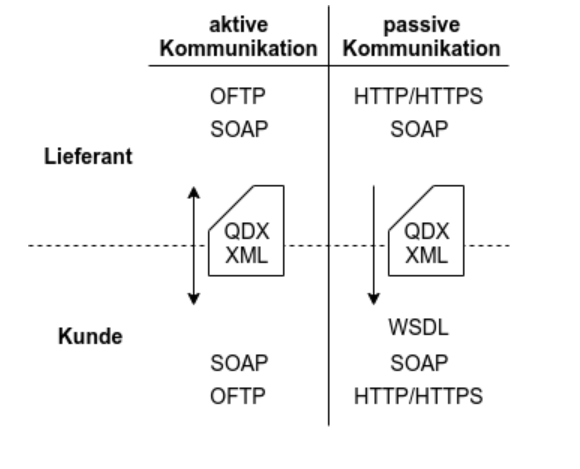
\includegraphics[width=8cm]{images/0x_requirement_analysis/qdx_communication_process}
\caption{QDX Communication Process}
\end{figure}

Das muss im Vorfeld auf beiden Seiten geklärt werden. Passive Kommunikation meint hierbei, dass der Schritt für die Initiierung stets auf der Lieferantenseite stattfindet\footnote{Quelle 2, S. 29: “Bei der „passiven“ Kommunikation ist also immer der Lieferant dafür verantwortlich, dass er die Daten des Kunden erhält und dass seine Daten an den Kunden übermittelt werden. Der Lieferant ist somit sowohl in der „Bring-“ als auch in der „Holschuld“.”}. Zu beachten ist hierbei, dass damit auch Veränderungen im Ablauf der Kommunikation entstehen. Insbesondere bedeutet es das zusätzliche Elemente für die Kommunikation benötigt werden (z. B. QDXComplaintList).
Bestimmte Dokumenteneingänge wie Beanstandungsmeldungen oder 8D-Reports müssen grundsätzlich von der Gegenseite über Acknowledge-Antworten bestätigt werden.
Nachfolgend werden Beispielabläufe für Beanstandungen in der aktiven sowie passiven Varianten dargestellt.

\begin{description}
\item [Variante aktive Kommunikation (über OFTP2)]\hfill
    \begin{enumerate}
        \item Lieferant <—QDXComplaint— Kunde
        \item Lieferant —QDXAcknowledgeComplaint—> Kunde
    \end{enumerate}
\item [Variante passive Kommunikation (über HTTP/HTTPS)]\hfill
    \begin{enumerate}
        \item Lieferant —QDXComplaintListRequest—> Kunde
        \item Lieferant <—QDXComplaintList— Kunde
        \item Lieferant —QDXComplaintRequest—> Kunde
        \item Lieferant <—QDXComplaint— Kunde
        \item Lieferant —QDXComplaintAcknowledgment—> Kunde
    \end{enumerate}
\end{description}

% Aufbau Datenpaket

% \begin{figure}[!h]
% \centering
% 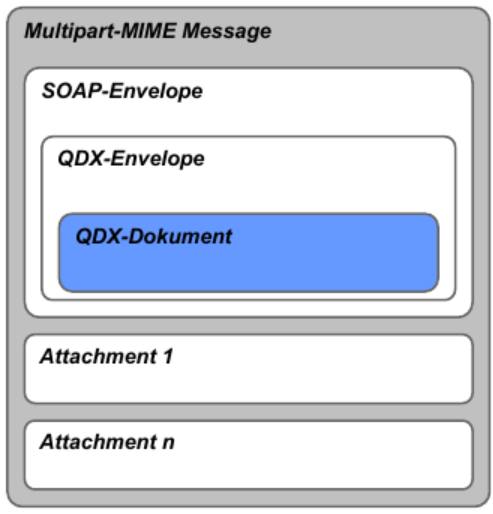
\includegraphics[width=7cm]{images/0x_requirement_analysis/qdx_message_structure.png}
% \caption{QDX Message Structure}
% \end{figure}

\subsubsection*{Vorteile}
\begin{itemize}
    \item Standard aus Verband der Automobilbranche e. V., es wird von vielen großen Autoherstellern und deren direkten Lieferanten genutzt
    \item Schema zur Validierung der Daten bereits verfügbar
    \item WSDL für den Complaint-Prozess enthalten
    \item Ausgereiftes Tooling für XML
\end{itemize}

\subsubsection*{Nachteile}
\begin{itemize}
    \item Technischer Unterbau wurde im Jahr 2005 entworfen
    \item Für einen reibungslosen Vorgang sind Abstimmungen mit den Lieferantensystemen nötig und für jeden Geschäftsprozess extra festzulegen (Leistungsmerkmale wie maximal zulässige Latenz, aktive/passive Kommunikation, etc.), denn diese werden von QDX nicht vorgegeben
    \item Unterschiedliche Kommunikationsweisen (aktiv/passiv) des Datenaustausches erfordern unterschiedliche Implementationen
    \item Die passive Kommunikation ist längst nicht so versatil wie die aktive Variante, weil ausschließlich die Lieferanten-Seite für die Übertragung und dem Beziehen von Daten verantwortlich ist
    \item Die Webservice-Variante erlaubt nur die unsichere Authentifizierung über Basic Authentication Header
    \item Für OFTP existieren vorwiegend kommerzielle Clients
    \item Lizenzgebühren für Nutzung in Softwareprodukte
    \item Einarbeitung in OFTP nötig
\end{itemize}

% Empfehlung
Da QDX beim aktuellen Kunden gegenwärtig nicht in Verwendung ist, wurde aus Gründen der Komplexität vorerst auf eine Einbindung verzichtet.
Falls es irgendwann doch dazu kommt, sollte man sich auf die Bestandteile des Formates konzentrieren die auch tatsächlich im operativen Geschäft beim Kunden benutzt werden.
Vermutlich am Ehesten alles bezogen auf Complaint-Prozesse plus 8D Reports.
Da sich die Dokumente an den realen Schriftverkehr bei Qualitätsbeanstandungen orientierte, könnte es Sinn ergeben sich bei der eigenen Modellierung durch die Überlegungen aus QDX inspirieren zu lassen.